\documentclass[journal]{IEEEtran}
\usepackage[english]{babel}

\usepackage{amssymb, amsmath} %Paquetes matemáticos de la American Mathematical 
\usepackage[utf8]{inputenc}
\usepackage{graphicx}
\usepackage{float}
\usepackage{hyperref}
\usepackage{listings}
\usepackage{xcolor}

\definecolor{codegreen}{rgb}{0,0.6,0}
\definecolor{codegray}{rgb}{0.5,0.5,0.5}
\definecolor{codepurple}{rgb}{0.58,0,0.82}
\definecolor{backcolour}{rgb}{0.95,0.95,0.92}
% Definicio de estilo para el codigo fuente que se cita
\lstdefinestyle{mystyle}{
    backgroundcolor=\color{backcolour},   
    commentstyle=\color{codegreen},
    keywordstyle=\color{magenta},
    numberstyle=\tiny\color{codegray},
    stringstyle=\color{codepurple},
    basicstyle=\ttfamily\footnotesize,
    breakatwhitespace=false,         
    breaklines=true,                 
    captionpos=b,                    
    keepspaces=true,
    numbers=left,                    
    numbersep=5pt,                  
    showspaces=false,                
    showstringspaces=false,
    showtabs=false,                  
    tabsize=2,
}
\lstset{style=mystyle}

\renewcommand{\lstlistingname}{Código}

\ifCLASSINFOpdf

\else

\fi
\begin{document}

\title{Ejercicio 3 - tema 7 \\ Administración de Redo log files}
%
\author{Vicente Romero Andrade}

\markboth{Ejercicio 3 - tema 7 Administración de Redo log files, Julio~2021}%
{Shell \MakeLowercase{\textit{et al.}}: }
% The only time the second header will appear is for the odd numbered pages

\maketitle


\IEEEpeerreviewmaketitle

\section{Objetivo}
% The very first letter is a 2 line initial drop letter followed

\IEEEPARstart{E}{l} objetivo es poner en práctica las tareas de administración 
básicas que se asocian con el mantenimiento de Redo Log files: 
Ubicación, tamaño, número de grupos y miembros.

\section{Desarrollo}
\subsection{sentencias}
\begin{lstlisting}[language=sql, caption=s-00-redologs.sql,label={lst:codigo1}]
  whenever sqlerror exit rollback
  set serveroutput on
  connect sys/system2 as sysdba
  --A
  !find /u0* -name redo*.log
  --B
  SELECT
         lf.GROUP#,
         l.SEQUENCE#,
         (BYTES/(1024*1024)) size_mb,
         BLOCKSIZE,
         MEMBERS,
         l.STATUS,
         min(FIRST_CHANGE#) MINIMO_SCN,
         min(FIRST_CHANGE#) FECHA_MINIMO_SCN,
         min(NEXT_CHANGE#) MAXIMO_SCN
  FROM v$logfile lf
      join v$log l on lf.GROUP#=l.GROUP#
  group by lf.GROUP#, l.SEQUENCE#, (BYTES/(1024*1024)), BLOCKSIZE, MEMBERS, l.STATUS;
  --C
  -- SE USA EL GRUPO 3
  --D
  SELECT
         lf.GROUP#,lf.STATUS,lf.TYPE,MEMBER
  FROM v$logfile lf
      join v$log l on lf.GROUP#=l.GROUP#;
  -- NULO SIGNIFICA QUE AUN SIGUE EN USO EL ARCHIVO, LOS OTROS ESTADOS SOLO HABLAN DE INDISPONIBILIDAD
  -- INVALID, STALE, DELETED
  -- E
  ALTER DATABASE 
    ADD LOGFILE GROUP 4(
      '/u01/app/oracle/oradata/VRABDA2/redo01_A.log',
      '/u01/app/oracle/oradata/VRABDA2/redo01_B.log')
      SIZE 50M BLOCKSIZE 512;
  
  ALTER DATABASE 
    ADD LOGFILE GROUP 5(
      '/u01/app/oracle/oradata/VRABDA2/redo02_A.log',
      '/u01/app/oracle/oradata/VRABDA2/redo02_B.log')
      SIZE 50M BLOCKSIZE 512;
  ALTER DATABASE 
    ADD LOGFILE GROUP 6(
      '/u01/app/oracle/oradata/VRABDA2/redo03_A.log',
      '/u01/app/oracle/oradata/VRABDA2/redo03_B.log')
      SIZE 50M BLOCKSIZE 512;
  -- F
  ALTER DATABASE
    ADD LOGFILE MEMBER '/u01/app/oracle/oradata/VRABDA2/redo01_C.log' TO GROUP 4;
  ALTER DATABASE
    ADD LOGFILE MEMBER '/u01/app/oracle/oradata/VRABDA2/redo02_C.log' TO GROUP 5;
  ALTER DATABASE
    ADD LOGFILE MEMBER '/u01/app/oracle/oradata/VRABDA2/redo03_C.log' TO GROUP 6;
  -- G 
  SELECT
         lf.GROUP#,
         l.SEQUENCE#,
         (BYTES/(1024*1024)) size_mb,
         BLOCKSIZE,
         MEMBERS,
         l.STATUS,
         min(FIRST_CHANGE#) MINIMO_SCN,
         min(FIRST_CHANGE#) FECHA_MINIMO_SCN,
         min(NEXT_CHANGE#) MAXIMO_SCN
  FROM v$logfile lf
      join v$log l on lf.GROUP#=l.GROUP#
  group by lf.GROUP#, l.SEQUENCE#, (BYTES/(1024*1024)), BLOCKSIZE, MEMBERS, l.STATUS;
  -- H
  -- Los archivos son inaccesibles ya que no han sido creados
  -- I
  -- J
  alter database clear logfile group 3;
  -- K
  alter database drop logfile group 1;
  alter database drop logfile group 2;
  alter database drop logfile group 3;
  --L
  ! find /u0* -name redo*0[1-3][a-c].log -exec rm {} \;
  --M
  !find /u0* -name redo*.log
  whenever sqlerror continue  
\end{lstlisting}
\begin{figure}[H]
  \centering
  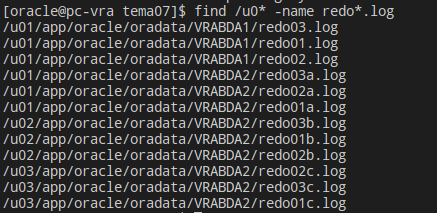
\includegraphics[scale=.22]{captura_1.png}
   \caption{Salida punto A}
   \label{fig:validador_1}
\end{figure}
\begin{figure}[H]
  \centering
  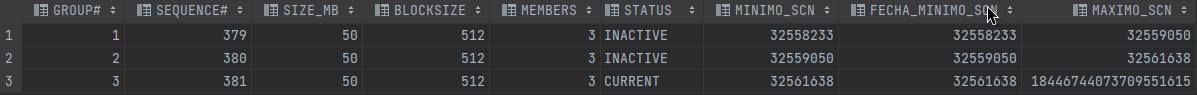
\includegraphics[scale=.20]{captura_2.png}
   \caption{Salida punto B}
   \label{fig:validador_2}
\end{figure}
\subsubsection{¿Qué grupo de Redo Log es el que se está empleando?}
Se usa el grupo 3
\subsubsection{¿Por qué razón el status de los miembros es nulo?}
Es nulo porque aun sigue en uso el archivo, los otros estados solo se refieren a estados 
de indisponibilidad por distintas causas.
\subsubsection{¿Qué otros valores del campo status pueden existir?}
\begin{itemize}
  \item Invalid
  \item Stale
  \item Deleted
\end{itemize}
\begin{figure}[H]
  \centering
  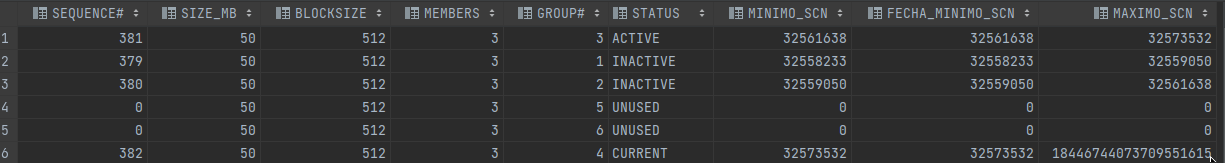
\includegraphics[scale=.20]{captura_5.png}
   \caption{Salida punto G}
   \label{fig:validador_4}
\end{figure}
Hay otros 3 grupos
\begin{figure}[H]
  \centering
  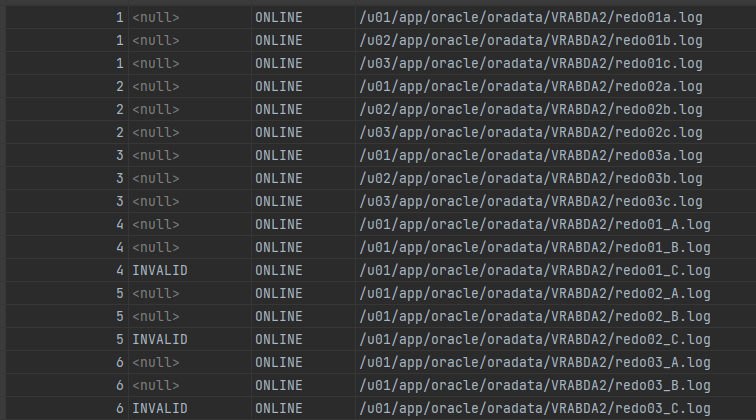
\includegraphics[scale=.20]{captura_4.png}
   \caption{Salida punto H}
   \label{fig:validador_5}
\end{figure}
Todos estan online pero hay 3 invalidos, esto es porque no tienen archivo creado
\begin{figure}[H]
  \centering
  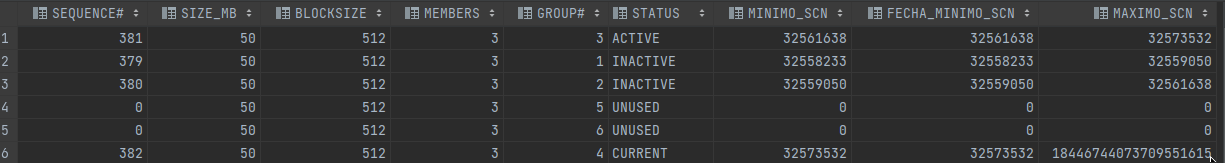
\includegraphics[scale=.20]{captura_5.png}
   \caption{Salida punto I}
   \label{fig:validador_6}
\end{figure}
\subsubsection{¿En qué status deberían estar para poder ser eliminados de forma segura?}
En Inactive o Unused
\begin{figure}[H]
  \centering
  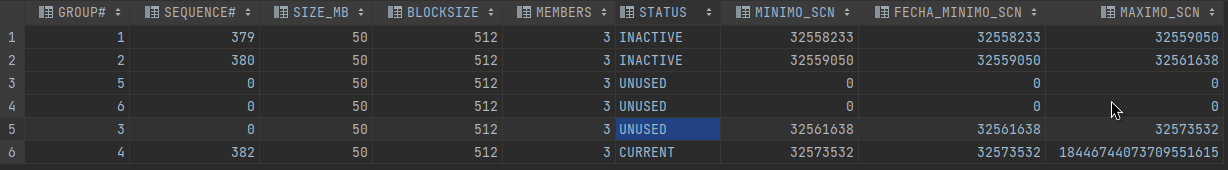
\includegraphics[scale=.20]{captura_6.png}
   \caption{Salida punto J}
   \label{fig:validador_7}
\end{figure}
\begin{figure}[H]
  \centering
  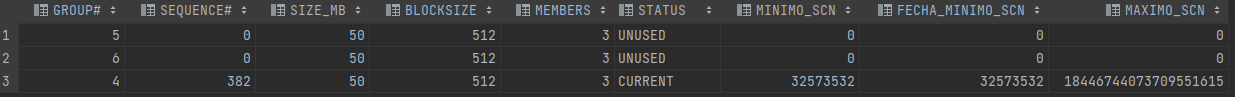
\includegraphics[scale=.20]{captura_7.png}
   \caption{Salida punto K}
   \label{fig:validador_8}
\end{figure}
\begin{figure}[H]
  \centering
  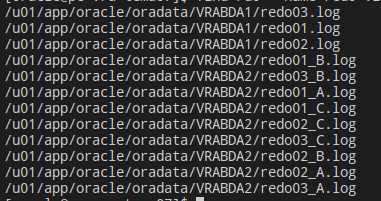
\includegraphics[scale=.25]{captura_8.png}
   \caption{Salida punto M}
   \label{fig:validador_9}
\end{figure}

\section{Conclusiones}
En este ejercicio se trabajo con los redo logs para reubicarlos, desactivarlos y eliminarlos 
o crearlos. Fue muy util poder hacer esto ya que se pueden mejorar los que existen por default para 
distintas necesidades.
\ifCLASSOPTIONcaptionsoff
  \newpage

\fi

\end{document}
